% =============================================================================
% IOPS for GysIO -- 20 minute presentation
% Compile with:  pdflatex iops_presentation.tex   (run twice for the outline/refs)
% =============================================================================
\documentclass[aspectratio=169,11pt]{beamer}

\usetheme{metropolis}

% ---- Fonts (Fira, pdflatex-friendly) ---------------------------------------
\usepackage[T1]{fontenc}
\usepackage[utf8]{inputenc}
\usepackage[sfdefault,scaled=.95]{FiraSans}
\usepackage{FiraMono}
\usepackage{newtxsf} % math in a sans style that blends with Fira

\usepackage{listings}
\usepackage{tcolorbox}
\usepackage{fontawesome5}
\usepackage{booktabs}
\usepackage{colortbl}
\usepackage{appendixnumberbeamer}  % backup slides excluded from the count
\usepackage{tikz}
\usetikzlibrary{positioning,arrows.meta,shapes.geometric,fit,backgrounds,decorations.pathreplacing,calc}

% ---- Palette: white + light blue, logo accents kept for code ---------------
\definecolor{iopsNavy}{HTML}{16323F}   % primary text (soft dark)
\definecolor{iopsBlue}{HTML}{1F8FD0}   % main accent (light blue)
\definecolor{iopsCyan}{HTML}{49B4E6}   % lighter blue
\definecolor{iopsSky}{HTML}{EAF5FC}    % very light blue fills / backgrounds
\definecolor{iopsPink}{HTML}{E0356E}   % code accent only
\definecolor{iopsGold}{HTML}{D99A00}   % code accent only
\definecolor{iopsGreen}{HTML}{6FA82B}  % code accent only
\definecolor{iopsGrey}{HTML}{6A7A86}   % muted captions
\definecolor{codeBg}{HTML}{F4FAFE}     % light-blue tinted code background

% ---- Metropolis colour overrides (light theme) -----------------------------
\setbeamercolor{normal text}{fg=iopsNavy, bg=white}
\setbeamercolor{background canvas}{bg=white}
\setbeamercolor{alerted text}{fg=iopsPink}
\setbeamercolor{example text}{fg=iopsGreen!75!black}
% White title with a light-blue progress rule underneath
\setbeamercolor{frametitle}{bg=white, fg=iopsNavy}
\setbeamercolor{progress bar}{fg=iopsBlue, bg=iopsSky}
\setbeamercolor{title separator}{fg=iopsBlue}
\setbeamercolor{progress bar in head/foot}{fg=iopsBlue, bg=iopsSky}
\setbeamercolor{progress bar in section page}{fg=iopsBlue, bg=iopsSky}
% Section pages and standout stay light instead of inverting to dark
\setbeamercolor{section title}{fg=iopsNavy}
\setbeamercolor{standout}{fg=iopsNavy, bg=iopsSky}
\metroset{progressbar=frametitle, sectionpage=none, numbering=fraction}

\setbeamertemplate{frametitle}[default][left]

% Keep the frame title flush-left with a little air above the rule
\setbeamerfont{frametitle}{size=\large, series=\bfseries}

% ---- Generic listings style ------------------------------------------------
\lstdefinestyle{base}{
  basicstyle=\ttfamily\footnotesize,
  backgroundcolor=\color{codeBg},
  frame=leftline,
  framerule=2pt,
  rulecolor=\color{iopsCyan},
  xleftmargin=10pt,
  framesep=6pt,
  aboveskip=4pt, belowskip=2pt,
  breaklines=true,
  showstringspaces=false,
  columns=fullflexible,
  keepspaces=true,
  numberstyle=\tiny\color{iopsGrey},
}

% YAML highlighting
\lstdefinelanguage{yaml}{
  keywords={true,false,null},
  keywordstyle=\color{iopsGold},
  comment=[l]{\#},
  commentstyle=\color{iopsGrey}\itshape,
  stringstyle=\color{iopsGreen!60!black},
  moredelim=[l][\color{iopsPink}\bfseries]{- },
  literate =
    {\{\{}{{\color{iopsCyan}\{\{}}2
    {\}\}}{{\color{iopsCyan}\}\}}}2,
}
\lstdefinestyle{yaml}{style=base,language=yaml,
  basicstyle=\ttfamily\fontsize{7.4}{8.6}\selectfont, columns=fixed}
\lstdefinestyle{py}{style=base,language=Python,
  keywordstyle=\color{iopsPink}\bfseries,
  commentstyle=\color{iopsGrey}\itshape,
  stringstyle=\color{iopsGreen!60!black}}
\lstdefinestyle{sh}{style=base,language=bash,
  keywordstyle=\color{iopsPink}\bfseries,
  commentstyle=\color{iopsGrey}\itshape,
  stringstyle=\color{iopsGreen!60!black},
  morekeywords={iops}}

% Inline code helper
\newcommand{\code}[1]{{\ttfamily\small\color{iopsNavy}#1}}
\newcommand{\hl}[1]{{\color{iopsPink}\bfseries #1}}

% Boxes
\newtcolorbox{keybox}[1][]{colback=iopsSky, colframe=iopsBlue,
  boxrule=0.6pt, arc=2pt, left=5pt, right=5pt, top=3pt, bottom=3pt, #1}

% Inline "chip" badge for listing domains
\newtcbox{\chip}{on line, colback=iopsSky, colframe=iopsBlue, boxrule=0.5pt,
  arc=3pt, left=3pt, right=3pt, top=1pt, bottom=1pt, fontupper=\footnotesize,
  nobeforeafter}

% Framed screenshot helpers (light-blue rounded border)
\newcommand{\shotW}[2]{\tikz\node[draw=iopsBlue, line width=0.6pt, inner sep=1pt,
  rounded corners=2pt]{\includegraphics[width=#1]{#2}};}
\newcommand{\shotH}[2]{\tikz\node[draw=iopsBlue, line width=0.6pt, inner sep=1pt,
  rounded corners=2pt]{\includegraphics[height=#1]{#2}};}

% Contributor photo (oval/circle crop with a light-blue ring)
% #1 = image file, #2 = name, #3 = affiliation, #4 = graphics opt (width=.. or height=..)
\newcommand{\person}[4]{%
  \begin{minipage}[t]{0.235\textwidth}\centering
    \begin{tikzpicture}
      \node[circle, draw=iopsBlue, line width=1pt, inner sep=0pt, minimum size=1.0cm,
        path picture={\node at (path picture bounding box.center)
          {\includegraphics[#4]{people/#1}};}]{};
    \end{tikzpicture}\\[1pt]
    {\scriptsize\bfseries #2}\\[-4pt]{\tiny\color{iopsGrey} #3}
  \end{minipage}}

% Section divider / transition slide: #1 = kicker, #2 = title, #3 = subtitle
% (not counted and not numbered, so the page fraction ignores dividers)
\newcommand{\divider}[3]{%
  {\setbeamertemplate{footline}{}%
  \begin{frame}[c,noframenumbering]{}
    \centering
    {\large\color{iopsGrey} #1}\par\vspace{6pt}
    {\Huge\bfseries\color{iopsNavy} #2}\par\vspace{10pt}
    {\color{iopsBlue}\rule{2.6cm}{1.5pt}}\par\vspace{8pt}
    {\footnotesize\color{iopsGrey} #3}
  \end{frame}}}

% ---- Title metadata --------------------------------------------------------
\title{IOPS}
\subtitle{Reproducible benchmarking, from one YAML to a report}
\date{June 2026 \quad\textperiodcentered\quad IOPS v3.5.6}
\author{Luan Teylo}
\institute{Integrated Orchestration for Parametric Studies}
\titlegraphic{\hfill
\includegraphics[height=2.4cm]{logo.png}}

\begin{document}

% =============================================================================
\maketitle

% =============================================================================
\section{Why IOPS}
% =============================================================================

\begin{frame}{The problem: one run is never enough}
  You want to know how \textsc{Gysela} writes to the PFS. So you ask:
  \begin{itemize}
    \item Which \hl{stripe count} gives the best write bandwidth?
    \item What about \hl{subfiling}?
    \item Does it hold at \hl{64 nodes} as well as 128? With more tasks per node?
    \item Is the gain \hl{stable}, or just one lucky run?
  \end{itemize}
  \pause
  \vspace{0.4em}
  In practice this becomes a pile of hand-edited scripts:
  \begin{columns}[T]
    \begin{column}{0.5\textwidth}
      \begin{itemize}
        \item one \code{sbatch} script per configuration
        \item copy/paste loops, magic suffixes
        \item \code{grep}/\code{awk} to scrape numbers
        \item a spreadsheet glued together by hand
      \end{itemize}
    \end{column}
    \begin{column}{0.5\textwidth}
      \begin{keybox}
        \faExclamationTriangle~Hard to reproduce, hard to share, easy to
        forget \emph{which} script produced \emph{which} number.
      \end{keybox}
    \end{column}
  \end{columns}
\end{frame}

\begin{frame}{The core idea}
  \begin{keybox}[colback=iopsSky, colframe=iopsBlue]
    \centering\large One YAML to rule them all.
  \end{keybox}
  \vspace{0.6em}
  \begin{columns}[T]
    \begin{column}{0.5\textwidth}
      \textbf{You write}
      \begin{itemize}
        \item the variables to sweep
        \item templates (run command / job script)
        \item a small Python parser
      \end{itemize}
    \end{column}
    \begin{column}{0.5\textwidth}
      \textbf{IOPS gives you}
      \begin{itemize}
        \item automatic execution (local or SLURM)
        \item a centralized CSV of results
        \item a nice interactive report
      \end{itemize}
    \end{column}
  \end{columns}
  \vspace{0.5em}
  \begin{center}
    \code{pip install iops-benchmark}\hfill
    {\footnotesize\color{iopsGrey}Python 3.10+, single tool, git-style subcommands}
  \end{center}
\end{frame}

\begin{frame}{The pipeline: one config, five stages}
  \centering
  \resizebox{\textwidth}{!}{%
  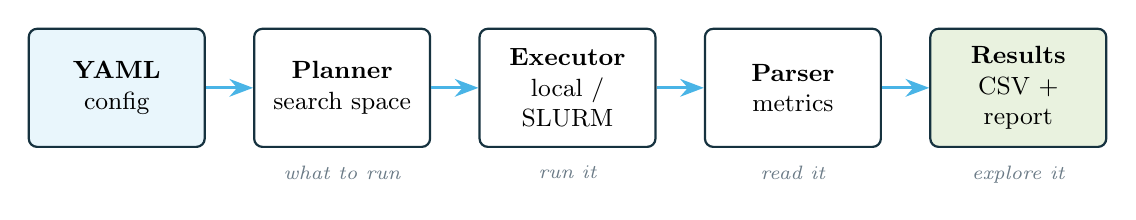
\begin{tikzpicture}[
      node distance=6mm,
      box/.style={rounded corners=3pt, draw=iopsNavy, line width=0.8pt,
        fill=white, text width=2.0cm, align=center, minimum height=1.5cm,
        font=\small},
      lab/.style={font=\scriptsize\itshape, color=iopsGrey},
      arr/.style={-{Stealth[length=3mm]}, line width=1pt, color=iopsCyan}]
    \node[box, fill=iopsCyan!12] (cfg) {\textbf{YAML}\\config};
    \node[box, right=of cfg] (plan) {\textbf{Planner}\\search space};
    \node[box, right=of plan] (exec) {\textbf{Executor}\\local / SLURM};
    \node[box, right=of exec] (parse) {\textbf{Parser}\\metrics};
    \node[box, right=of parse, fill=iopsGreen!15] (out) {\textbf{Results}\\CSV + report};
    \draw[arr] (cfg) -- (plan);
    \draw[arr] (plan) -- (exec);
    \draw[arr] (exec) -- (parse);
    \draw[arr] (parse) -- (out);
    \node[lab, below=1mm of plan] {what to run};
    \node[lab, below=1mm of exec] {run it};
    \node[lab, below=1mm of parse] {read it};
    \node[lab, below=1mm of out] {explore it};
  \end{tikzpicture}}

  \vspace{0.9em}
  \begin{keybox}
    The \hl{cache} sits underneath all of this: a result, once computed, is
    never computed again, and can be \emph{reused} when the study grows.
  \end{keybox}
\end{frame}

% =============================================================================
\section{The config file}
% =============================================================================

\divider{Part 1}{Describe the experiment}{benchmark \textperiodcentered\ vars \textperiodcentered\ command \textperiodcentered\ scripts \textperiodcentered\ output}

\begin{frame}[fragile]{The smallest useful config (IOR)}
  \begin{columns}[T]
    \begin{column}{0.64\textwidth}
\begin{lstlisting}[style=yaml,basicstyle=\ttfamily\fontsize{5.3}{6.3}\selectfont,columns=fixed]
benchmark:
  name: "IOR sweep"
  workdir: "./workdir"
  executor: "local"
  repetitions: 3

vars:
  block_size:               # 3 values
    type: int
    sweep: { mode: list, values: [256, 512, 1024] }
  transfer_size:            # 2 values
    type: int
    sweep: { mode: list, values: [1, 4] }

command:
  template: "ior -w -b {{ block_size }}m -t {{ transfer_size }}m"

scripts:
  - name: ior
    script_template: |
      #!/bin/bash
      mpirun -np 4 {{ command.template }}
    parser:
      parser_script: |
        def parse(p):
            ...

output:
  sink: { type: csv }       # csv, parquet, or sqlite
\end{lstlisting}
    \end{column}
    \begin{column}{0.36\textwidth}
      Five required sections:
      \begin{itemize}
        \item \code{benchmark}: where \& how
        \item \code{vars}: the space
        \item \code{command}: the run
        \item \code{scripts}: job + parser
        \item \code{output}: the sink
      \end{itemize}
      \vspace{0.4em}
      \begin{keybox}
        \faInfoCircle~By default IOPS runs \hl{every combination}:\\[2pt]
        \code{3 x 2 = 6} configs $\times$ 3 reps = \hl{18 runs}, a script
        generated for each.
      \end{keybox}
    \end{column}
  \end{columns}
\end{frame}

% =============================================================================
\section{vars: the search space}
% =============================================================================

\begin{frame}[fragile]{How a variable gets its value}
  \begin{columns}[T]
    \begin{column}{0.58\textwidth}
\begin{lstlisting}[style=yaml]
vars:
  # 1. SWEPT - the axes of the study
  nodes:
    type: int
    sweep: { mode: list, values: [1, 2, 4, 8] }
  ppn:
    type: int
    sweep: { mode: range, start: 8, stop: 32, step: 8 }

  # 2. DERIVED - computed from others (Jinja2)
  ntasks:
    type: int
    expr: "{{ nodes * ppn }}"

  # 3. CONSTANT - a literal expr, fixed for all runs
  block_size:
    type: int
    expr: "1024"
\end{lstlisting}
    \end{column}
    \begin{column}{0.42\textwidth}
      \begin{itemize}
        \item \hl{sweep} defines the axes\\ (\code{list} or \code{range})
        \item \hl{expr} derives a value\\ with full Jinja2
        \item a literal \hl{expr} = constant
      \end{itemize}
      \vspace{0.4em}
      The matrix is the \emph{cross-product} of the swept axes:
      \begin{center}
        \code{4 nodes x 3 ppn = 12} points\\(x repetitions)
      \end{center}
    \end{column}
  \end{columns}
\end{frame}

\begin{frame}[fragile]{Conditional variables: sweep only when relevant}
  A variable can be swept only \hl{when} another makes it meaningful, with a
  \code{default} otherwise:
  \begin{columns}[T]
    \begin{column}{0.6\textwidth}
\begin{lstlisting}[style=yaml,basicstyle=\ttfamily\fontsize{6.6}{7.8}\selectfont,columns=fixed]
vars:
  use_compression:
    type: bool
    sweep: { mode: list, values: [true, false] }
  compression_level:
    type: int
    sweep: { mode: list, values: [1, 5, 9] }
    when: "use_compression"   # only when true
    default: 0                # otherwise fixed

command:                      # full Jinja2 in templates
  template: >
    mybench {% if use_compression %}
    --zlevel {{ compression_level }}{% endif %}
\end{lstlisting}
    \end{column}
    \begin{column}{0.4\textwidth}
      \begin{keybox}
        \faInfoCircle~Without \code{when}: $2\times3 = 6$ runs, half
        redundant.\\[3pt]
        With \code{when}: $3 + 1 = 4$ runs (the three levels, plus one
        ``no compression'').
      \end{keybox}
      \vspace{0.4em}
      \begin{keybox}[colback=iopsGreen!10, colframe=iopsGreen]
        \faCode~Templates get the \hl{full Jinja2}: \code{\{\% if \%\}}, loops,
        filters, expressions.
      \end{keybox}
    \end{column}
  \end{columns}
\end{frame}

\begin{frame}[fragile]{Constraints: drop combinations that make no sense}
  Filter out invalid points before anything runs (here: IOR needs
  \code{block\_size} to be a multiple of \code{transfer\_size}):
\begin{lstlisting}[style=yaml]
constraints:
  - name: block_alignment
    rule: "block_size % transfer_size == 0"
    violation_policy: skip       # skip | warn | error
\end{lstlisting}
  \begin{keybox}
    \faInfoCircle~The \code{rule} is any boolean expression over your variables;
    violations are \code{skip}ped (or \code{warn}/\code{error}). 
  \end{keybox}
\end{frame}

% =============================================================================
\section{Exploring the space}
% =============================================================================

\begin{frame}{You do not always want the full cross-product}
  \begin{center}
  \begin{tabular}{@{}lllc@{}}
    \toprule
    \textbf{Method} & \textbf{Coverage} & \textbf{Best for} & \textbf{Deterministic?} \\
    \midrule
    \rowcolor{iopsCyan!10}
    \code{exhaustive} & every combination & small spaces, full picture & yes \\
    \code{random}     & sampled subset    & large spaces, statistics & seed \\
    \rowcolor{iopsGold!15}
    \code{bayesian}   & guided to optimum & expensive runs, find best & no \\
    \code{adaptive}   & step to a limit   & find a threshold / cliff & yes \\
    \bottomrule
  \end{tabular}
  \end{center}
  \vspace{0.6em}
  \begin{keybox}
    \faSlidersH~Switch strategy with \emph{one line} (\code{search\_method}):
    the rest of the config is untouched.
  \end{keybox}
\end{frame}

\begin{frame}[fragile]{Bayesian: find the best I/O setting cheaply}
  \begin{columns}[c]
    \begin{column}{0.46\textwidth}
\begin{lstlisting}[style=yaml]
benchmark:
  search_method: "bayesian"
  bayesian_config:
    objective_metric: "bandwidth"
    objective: "maximize"
    n_initial_points: 5
    n_iterations: 20
\end{lstlisting}
      \footnotesize IOPS builds a surrogate model of the \code{objective\_metric}
      and \hl{spends runs where they pay off}, instead of testing everything.
      \vspace{0.4em}
      \begin{keybox}[colback=iopsGold!12, colframe=iopsGold]
        \faBullseye~$\sim$90\% of the optimum after only $\sim$7\% of the
        space.\\[2pt]
        {\scriptsize\urlstyle{same}More details:
        \url{https://iops.gitlabpages.inria.fr/blog/bayesian-optimization-study/}}
      \end{keybox}
    \end{column}
    \begin{column}{0.54\textwidth}
      \centering
      \shotW{\linewidth}{figures/node_selection.png}

      \vspace{3pt}
      {\footnotesize\color{iopsGrey} Bayesian (centre/right) quickly concentrates
      on \code{nodes=64} (green = fast configs); random (left) keeps sampling
      everywhere.}
    \end{column}
  \end{columns}
\end{frame}

\begin{frame}[fragile]{exhaustive\_vars: never miss a value}
  Search the expensive axes, but \hl{fully sweep} the one knob you study:
\begin{lstlisting}[style=yaml,basicstyle=\ttfamily\fontsize{7.7}{9.2}\selectfont,columns=fixed]
benchmark:
  search_method: "bayesian"   # or "random"
  exhaustive_vars: ["stripe_count"]
vars:
  nodes:
    sweep: { values: [1, 2, 4, 8] }     # searched by BO
  ppn:
    sweep: { values: [16, 32] }         # searched by BO
  stripe_count:
    sweep: { values: [1, 2, 4, 8] }     # fully run at each point
\end{lstlisting}
  \vspace{0.4em}
  \begin{columns}[c]
    \begin{column}{0.5\textwidth}
      \footnotesize
      \begin{tabular}{@{}lll@{}}
        \toprule
        \textbf{BO picks} & \textbf{IOPS runs} & \textbf{Back to BO} \\
        \midrule
        \rowcolor{iopsCyan!10}
        nodes=4, ppn=16 & stripe=1,2,4,8 & best write\_bw \\
        nodes=8, ppn=32 & stripe=1,2,4,8 & best write\_bw \\
        \bottomrule
      \end{tabular}
    \end{column}
    \begin{column}{0.5\textwidth}
      \begin{keybox}[colback=iopsGreen!10, colframe=iopsGreen]
        \faCogs~BO picks a \code{(nodes, ppn)} point; IOPS runs \emph{all}
        \code{stripe\_count} values (kept for the report). BO is told only the
        \hl{best} per point.
      \end{keybox}
    \end{column}
  \end{columns}
\end{frame}

% =============================================================================
\section{command \& scripts}
% =============================================================================

\begin{frame}[fragile]{Metrics: the numbers IOPS measures}
  A \hl{metric} is a named measurement. You \hl{declare} it in YAML and a
  \code{parse()} \hl{produces} it from the output (IOR):
\begin{lstlisting}[style=yaml]
parser:
  file: "{{ execution_dir }}/stdout"
  metrics:                       # declare what you measure
    - { name: write_bw, type: float }
    - { name: read_bw,  type: float }
  parser_script: |
    import re
    def parse(path):
        text = open(path).read()
        write = re.search(r"Max Write:\s+([\d.]+)", text).group(1)
        read  = re.search(r"Max Read:\s+([\d.]+)",  text).group(1)
        return {"write_bw": float(write), "read_bw": float(read)}
\end{lstlisting}
  \begin{keybox}
    \faInfoCircle~Metrics are IOPS's currency: they become \code{results.csv}
    columns and report plots, and drive the Bayesian \code{objective\_metric}
    and adaptive \code{stop\_when}. The keys returned by \code{parse()} must
    match the declared names.
  \end{keybox}
\end{frame}




% =============================================================================
\section{output: the results}
% =============================================================================

\begin{frame}[fragile]{output: where the results go}
  One \code{output.sink} gathers every parsed metric into a single dataset:
\begin{lstlisting}[style=yaml]
output:
  sink:
    type: csv                 # csv, parquet, or sqlite
    path: "{{ workdir }}/results.csv"
\end{lstlisting}
  \begin{columns}[T]
    \begin{column}{0.5\textwidth}
      \begin{itemize}
        \item one row per (config, repetition)
        \item all variables \emph{and} metrics as columns
        \item results are always \hl{appended}
      \end{itemize}
    \end{column}
    \begin{column}{0.5\textwidth}
      \begin{keybox}
        \faTable~Formats: \code{csv}, \code{parquet}, \code{sqlite}. You choose
        where it lives: ready to plot or diff.
      \end{keybox}
    \end{column}
  \end{columns}
\end{frame}

% =============================================================================
\section{Running it}
% =============================================================================

\divider{Part 2}{Run it and see the results}{dry-run \textperiodcentered\ run \textperiodcentered\ watch \textperiodcentered\ report}

\begin{frame}[fragile]{Preview the plan before running}
\begin{lstlisting}[style=sh]
iops run cfg.yaml --dry-run --time-estimate "60,120,300"
\end{lstlisting}
  \begin{columns}[c]
    \begin{column}{0.38\textwidth}
      A dry run reports, without launching anything:
      \begin{itemize}
        \item how many \hl{tests} and \hl{executions}
        \item estimated \hl{core-hours} and wall-clock
        \item a \hl{scenario} table for different per-run times
      \end{itemize}
    \end{column}
    \begin{column}{0.62\textwidth}
      \centering\shotH{8cm}{figures/dryrun.png}
    \end{column}
  \end{columns}
\end{frame}

\begin{frame}[fragile]{Run: one command, a tidy workdir}
\begin{lstlisting}[style=sh]
iops run cfg.yaml               # execute the plan
\end{lstlisting}
  \vspace{0.2em}
  \begin{columns}[T]
    \begin{column}{0.58\textwidth}
\begin{lstlisting}[style=sh,basicstyle=\ttfamily\fontsize{7.4}{8.8}\selectfont,columns=fixed]
run_001/
  exec_0001/            # one folder per config
    repetition_001/
      run_ior.sh        # the script that ran
      stdout  stderr    # captured output
      ior.out           # benchmark output
  results.csv           # parsed metrics
  report.html           # interactive report
\end{lstlisting}
    \end{column}
    \begin{column}{0.42\textwidth}
      \begin{keybox}
        \faFolderOpen~Fully \hl{reproducible}: the script that produced each
        number sits right next to its \code{stdout}, \code{stderr}, and output
        files.
      \end{keybox}
    \end{column}
  \end{columns}
\end{frame}

\begin{frame}[fragile]{Watch it run, live}
\begin{lstlisting}[style=sh]
iops find run_001 --watch      # live table + progress bar
\end{lstlisting}
  \centering
  \shotW{0.85\textwidth}{figures/watch.png}

  %\vspace{0.3em}
  {\footnotesize\color{iopsGrey} Per-execution status and metrics update in
  place, with a progress bar and core-hours used.}
\end{frame}

\begin{frame}[fragile]{From CSV to an interactive report}
\begin{lstlisting}[style=sh]
iops report run_001            # one self-contained HTML file
\end{lstlisting}
  \begin{columns}[c]
    \begin{column}{0.38\textwidth}
      The report bundles:
      \begin{itemize}
        \item summary \hl{statistics} per metric
        \item the \hl{best configurations} found
        \item the \hl{search space} explored
        \item interactive \hl{plots}
      \end{itemize}
    \end{column}
    \begin{column}{0.62\textwidth}
      \centering\shotH{6.6cm}{figures/report01.png}
    \end{column}
  \end{columns}
\end{frame}

\begin{frame}{Report: explore the search}
  \centering
  \shotW{0.92\textwidth}{figures/report02.png}

  \vspace{0.4em}
  {\footnotesize\color{iopsGrey} Interactive Plotly charts: scatter, bars,
  heatmaps, parallel coordinates, and search-evolution views.}
\end{frame}

\begin{frame}[fragile]{Make the report part of the config}
  Add a \code{reporting} section and the report is generated automatically after
  every run, with exactly the plots you care about:
\begin{lstlisting}[style=yaml]
reporting:
  enabled: true
  metrics:
    write_bw:
      plots:
        - { type: bar,     x: stripe_count }       # write_bw vs stripe count
        - { type: heatmap, x: nodes, y: ppn }
\end{lstlisting}
  \begin{keybox}[colback=iopsGreen!10, colframe=iopsGreen]
    \faChartLine~A single bar chart of \code{write\_bw} vs \code{stripe\_count}
    answers ``which stripe count wins?'' at a glance, refreshed every time the
    study runs.
  \end{keybox}
\end{frame}

% =============================================================================
\section{Resource probes}
% =============================================================================

\divider{Part 3}{Going further}{probes \textperiodcentered\ caching}

\begin{frame}[fragile]{Resource probes: CPU, memory, GPU}
  \begin{columns}[T]
    \begin{column}{0.5\textwidth}
      Turn on lightweight samplers to record the \hl{resource footprint} of each
      run:
\begin{lstlisting}[style=yaml]
benchmark:
  probes:
    resource_sampling: true   # CPU + memory
    gpu_sampling: true        # GPU (nvidia-smi)
    sampling_interval: 1.0    # seconds
\end{lstlisting}
      \begin{itemize}
        \item low-priority sampler \hl{per node}
        \item per-core CPU \%, memory, GPU use
        \item folded into the report as heatmaps
      \end{itemize}
      \begin{keybox}[colback=iopsGold!12, colframe=iopsGold]
        \faThermometerHalf~Sampling adds a little overhead: take a
        \hl{baseline} first, then enable probes.
      \end{keybox}
    \end{column}
    \begin{column}{0.5\textwidth}
      \centering
      \shotH{6.4cm}{figures/cpu_overhead_heatmap.png}

      \vspace{2pt}
      {\footnotesize\color{iopsGrey} CPU-usage overhead per configuration
      (sampling vs.\ baseline).}
    \end{column}
  \end{columns}
\end{frame}

% =============================================================================
\section{Scale \& reuse}
% =============================================================================



\begin{frame}[fragile]{Caching: never compute the same point twice}
  \begin{columns}[T]
    \begin{column}{0.55\textwidth}
\begin{lstlisting}[style=yaml]
benchmark:
  cache_file: "./workdir/iops_cache.db"
  cache_exclude_vars: ["output_file"]  # path-like
\end{lstlisting}
\begin{lstlisting}[style=sh]
iops run cfg.yaml --use-cache   # skip cached
iops cache stats  cache.db
iops cache list   cache.db nodes=8
\end{lstlisting}
    \end{column}
    \begin{column}{0.45\textwidth}
      \begin{itemize}
        \item key = \hl{parameter values} + repetition
        \item only \code{SUCCEEDED} runs cached
        \item retry failures safely
      \end{itemize}
      \begin{keybox}[colback=iopsPink!8, colframe=iopsPink]
        \faExclamationTriangle~The key is the \emph{parameters}, not the
        command. Change the command's behaviour $\Rightarrow$ clear the cache or
        bump a \code{cache\_version} var.
      \end{keybox}
    \end{column}
  \end{columns}
\end{frame}



% =============================================================================
\section{Wrap-up}
% =============================================================================

\begin{frame}{Not only I/O}
  IOPS \textbf{started as an I/O benchmarking tool} (IOR, MDTEST, IO500), then we
  made the engine \hl{generic}. It is a working, fully documented tool with
  \hl{growing adoption} beyond its original scope:

  \vspace{0.5em}
  \begin{columns}[t]
    \begin{column}{0.32\textwidth}
      \begin{keybox}[equal height group=adopt]
        {\color{iopsBlue}\faServer~\textbf{CEA \textperiodcentered\ NUMPEX}}\\[4pt]
        {\footnotesize Parametric performance studies on production HPC systems.}
      \end{keybox}
    \end{column}
    \begin{column}{0.32\textwidth}
      \begin{keybox}[equal height group=adopt]
        {\color{iopsBlue}\faTrophy~\textbf{IO500 collaboration}}\\[4pt]
        {\footnotesize INRIA, JGU, Sandia, and the IO500 community: smart
        parameter-space search to optimize IO500 scores.}
      \end{keybox}
    \end{column}
    \begin{column}{0.32\textwidth}
      \begin{keybox}[equal height group=adopt]
        {\color{iopsBlue}\faIndustry~\textbf{INRIA (Concace) \textperiodcentered\ Airbus}}\\[4pt]
        {\footnotesize Under evaluation for industrial HPC performance studies.}
      \end{keybox}
    \end{column}
  \end{columns}

  \vspace{0.5em}
  \begin{keybox}[colback=white]
    \faLightbulb~If it runs from a script and prints a number, IOPS can sweep it,
    schedule it, cache it, and plot it, whatever the domain.
  \end{keybox}
\end{frame}

\begin{frame}{Get involved}
  \centering
  \begin{keybox}[width=0.95\textwidth, top=2pt, bottom=2pt]
    \centering
    {\footnotesize IOPS is an open-source project created at \textbf{TADaaM} (Inria).}\\[2pt]
    {\scriptsize\faGlobe~\href{https://iops.gitlabpages.inria.fr/}{iops.gitlabpages.inria.fr}
    \;\textbar\;
    \faGitlab~\href{https://gitlab.inria.fr/lgouveia/iops}{gitlab.inria.fr/lgouveia/iops}
    \;\textbar\;
    \faBox~{\ttfamily pip install iops-benchmark}}\\[2pt]
    {\footnotesize Want to use, contribute, or share ideas? Email
    \href{mailto:luan.teylo@inria.fr}{luan.teylo@inria.fr} or open an issue.}
  \end{keybox}

  \vspace{1pt}
  {\footnotesize\color{iopsGrey}\textbf{Contributors}}\par
  \vspace{1pt}
  \person{luan_teylo.png}{Luan Teylo}{Inria}{height=1.4cm}\hfill
  \person{francieli_boito.png}{Francieli Boito}{Inria}{width=1.4cm}\hfill
  \person{Abdraman_mahamat.png}{Abdraman Mahamat}{Inria}{height=1.4cm}\hfill
  \person{mihail_popov.jpeg}{Mihail Popov}{Inria}{width=1.4cm}\par
  \vspace{1pt}
  \person{meline_trochon.png}{M\'eline Trochon}{Inria/DDN}{height=1.4cm}\hfill
  \person{jerome_charousset.png}{J\'er\^ome Charousset}{CEA}{height=1.4cm}\hfill
  \person{alexandre_lou-poueyou.png}{Alexandre Lou-Poueyou}{Inria}{height=1.4cm}\hfill
  \person{almousa_mohamad.png}{Mohamad Almousa}{Inria}{height=1.4cm}
\end{frame}

\appendix

% =============================================================================
\section{Backup}
% =============================================================================

\divider{}{Extra}{parallel execution \textperiodcentered\ adaptive \textperiodcentered\ growing the search space \textperiodcentered\ multi-machine \textperiodcentered\ SLURM \textperiodcentered\ CI/CD \textperiodcentered\ archive}

\begin{frame}[fragile]{Parallel execution}
  By default tests run one at a time. One setting changes that:
\begin{lstlisting}[style=yaml]
benchmark:
  parallel: 4        # up to 4 tests concurrently
\end{lstlisting}
  \code{iops run cfg.yaml -{}-parallel 4}\quad (CLI overrides YAML)
  \vspace{0.5em}
  \begin{center}
  \begin{tabular}{@{}lll@{}}
    \toprule
    \textbf{Method} & \textbf{Max parallelism} & \textbf{Why} \\
    \midrule
    \code{exhaustive} / \code{random} & unlimited & tests are independent \\
    \code{bayesian}  & 1 & each result feeds the next suggestion \\
    \code{adaptive}  & \#probes & probes independent, steps sequential \\
    \bottomrule
  \end{tabular}
  \end{center}
  \vspace{0.4em}
  \begin{keybox}
    Works with \emph{both} backends: parallel subprocesses locally, or many
    SLURM jobs submitted and polled at once. Budget tracking stays accurate.
  \end{keybox}
\end{frame}

\begin{frame}[fragile]{Growing the parameter space without re-running}
  You ran a full sweep. Now you want to add a \emph{new} axis,
  \code{compression}, but keep the old results for \code{compression=off}.
\begin{lstlisting}[style=sh,basicstyle=\ttfamily\scriptsize]
# Add a constant variable to every existing cache entry
iops cache rebuild cache.db --add compression:bool=false -o new_cache.db
\end{lstlisting}
\begin{lstlisting}[style=yaml]
vars:
  nodes:       { type: int,  sweep: { mode: list, values: [1, 2, 4, 8] } }
  compression: { type: bool, sweep: { mode: list, values: [false, true] } }
\end{lstlisting}
  \begin{keybox}[colback=iopsGreen!10, colframe=iopsGreen]
    \faMagic~Now \code{iops run --use-cache} finds hits for all
    \code{compression=false} points and only runs the \emph{new}
    \code{compression=true} half. The old runs are reused, not repeated.
  \end{keybox}
\end{frame}

\begin{frame}{Catch regressions when commits land}
  \begin{center}
  \resizebox{\textwidth}{!}{%
  \begin{tikzpicture}[node distance=6mm,
      b/.style={rounded corners=3pt, draw=iopsNavy, line width=0.8pt, fill=white,
        align=center, font=\small, minimum height=1.0cm, text width=2.4cm},
      arr/.style={-{Stealth[length=3mm]}, line width=1pt, color=iopsCyan}]
    \node[b, fill=iopsCyan!12] (push) {new commit};
    \node[b, right=of push] (ci) {CI job\\\code{iops run -{}-machine ci}};
    \node[b, right=of ci] (cache) {append to\\\code{history.csv}};
    \node[b, right=of cache, fill=iopsGreen!15] (cmp) {compare vs\\baseline};
    \node[b, right=of cmp, fill=iopsPink!15] (gate) {\faFlag~pass\\or fail};
    \draw[arr] (push)--(ci); \draw[arr] (ci)--(cache);
    \draw[arr] (cache)--(cmp); \draw[arr] (cmp)--(gate);
  \end{tikzpicture}}
  \end{center}
  \vspace{0.3em}
  \begin{enumerate}
    \item On each new commit, the CI job runs the \emph{same} config with the
      small \code{ci} profile.
    \item Results \hl{append} to a central \code{history.csv}, building a record
      over time.
    \item Compare against the baseline; \hl{fail the pipeline} if the metric
      regresses beyond a threshold.
  \end{enumerate}
\end{frame}

\begin{frame}[fragile]{A CI machine profile + pipeline}
  \begin{columns}[T]
    \begin{column}{0.5\textwidth}
      A fast \code{ci} profile that writes to a \hl{central CSV}:
\begin{lstlisting}[style=yaml]
machines:
  ci:
    benchmark:
      repetitions: 1
    vars:
      nodes:
        sweep: { values: [1, 4, 8] }
    output:
      sink:
        type: csv
        path: "/shared/iops/history.csv"
\end{lstlisting}
    \end{column}
    \begin{column}{0.5\textwidth}
\begin{lstlisting}[style=sh]
# .gitlab-ci.yml (sketch)
io-benchmark:
  rules:
    - if: $CI_PIPELINE_SOURCE ==
          "merge_request_event"
  script:
    - pip install iops-benchmark
    - iops run cfg.yaml --machine ci
    - python compare.py
        /shared/iops/history.csv
\end{lstlisting}
    \end{column}
  \end{columns}
  \begin{keybox}
    \faRocket~You decide where results live: every commit \hl{appends} to one
    \code{history.csv}, so performance over time sits in a single file you can
    diff. (\code{IOPS\_MACHINE=ci} works too.)
  \end{keybox}
\end{frame}

\begin{frame}[fragile]{The SLURM backend (and beyond)}
  \begin{columns}[T]
    \begin{column}{0.58\textwidth}
\begin{lstlisting}[style=yaml,basicstyle=\ttfamily\fontsize{6.8}{8}\selectfont,columns=fixed]
benchmark:
  executor: "slurm"
  cores_expr: "{{ nodes * ppn }}"
  max_core_hours: 1000          # budget guard
  slurm_options:
    commands:                   # override the defaults
      submit: "sbatch"
      status: "squeue -j {job_id} --format=%T"
      info:   "scontrol show job {job_id}"
      cancel: "scancel {job_id}"
    poll_interval: 30           # seconds
\end{lstlisting}
    \end{column}
    \begin{column}{0.42\textwidth}
      IOPS handles the lifecycle:
      \begin{itemize}
        \item submit, poll, status
        \item per-job status tracking
        \item core-hour budget
      \end{itemize}
      \vspace{0.3em}
      \begin{keybox}[colback=iopsGreen!10, colframe=iopsGreen]
        \faSlidersH~Swap these for \emph{any} scheduler or wrapper (the
        \code{\{job\_id\}} placeholder is filled at runtime). Not tied to SLURM.
      \end{keybox}
    \end{column}
  \end{columns}
\end{frame}

\begin{frame}[fragile]{Archiving a run}
  Bundle a whole run into one portable, checksummed archive to share or back up:
\begin{lstlisting}[style=sh]
iops archive create ./workdir/run_001 -o study.tar.gz  # pack a run
iops archive extract study.tar.gz -o ./extracted       # unpack it
iops find study.tar.gz                                  # inspect, no extract
\end{lstlisting}
  \begin{keybox}
    \faBoxOpen~The archive carries a \hl{manifest} and \hl{checksums}, so a study
    stays self-contained and verifiable when moved between machines.
  \end{keybox}
\end{frame}

\begin{frame}[fragile]{Multi-machine support}
  The \hl{same experiment} on different clusters, in \hl{one file}: override only
  the site-specific setup.
  \begin{columns}[c]
    \begin{column}{0.4\textwidth}
\begin{lstlisting}[style=yaml,basicstyle=\ttfamily\fontsize{6.4}{7.6}\selectfont,columns=fixed]
# Base: the experiment,
# shared by every machine
benchmark:
  workdir: "./workdir"
  repetitions: 5
vars:
  nodes:
    sweep: { values: [1,2,4,8] }
  ppn:
    sweep: { values: [16,32] }
command:
  template: "ior -w -b 1g -t 2m"
\end{lstlisting}
    \end{column}
    \begin{column}{0.05\textwidth}
      \centering
      {\Large\color{iopsBlue}$\cdots$}\\[2pt]
      {\tiny\color{iopsGrey}same\\file}
    \end{column}
    \begin{column}{0.55\textwidth}
\begin{lstlisting}[style=yaml,basicstyle=\ttfamily\fontsize{6.3}{7.6}\selectfont,columns=fixed]
machines:            # only the site-specific setup differs
  plafrim:
    benchmark: { workdir: "/scratch/$USER/b" }
    scripts:
      - name: run
        script_template: |
          #SBATCH --partition=bora
          module load openmpi
          srun {{ command.template }}
  grid5000:                            # OAR, not SLURM
    benchmark: { workdir: "/home/$USER/b" }
    scripts:
      - name: run
        script_template: |
          #OAR -l nodes={{ nodes }},walltime=1:00:00
          module load openmpi
          mpirun {{ command.template }}
\end{lstlisting}
    \end{column}
  \end{columns}
\begin{lstlisting}[style=sh,basicstyle=\ttfamily\scriptsize]
iops run config.yaml --machine plafrim     # run on PlaFRIM
iops run config.yaml --machine grid5000    # run on Grid'5000
\end{lstlisting}
\end{frame}

\begin{frame}[fragile]{Adaptive: probe for a limit}
  When the question is \emph{``how far can we push it?''} rather than
  \emph{``which is best?''}:
  \begin{columns}[T]
    \begin{column}{0.54\textwidth}
\begin{lstlisting}[style=yaml,basicstyle=\ttfamily\fontsize{6}{7.1}\selectfont,columns=fixed]
benchmark:
  search_method: "adaptive"
vars:
  nodes:                          # swept as usual
    type: int
    sweep: { mode: list, values: [1, 2, 4] }
  problem_size:
    type: int
    adaptive:
      initial: 1000
      factor: 2                     # double each step
      stop_when: "exit_code != 0"   # until it breaks
      max_iterations: 15            # safety net
\end{lstlisting}
    \end{column}
    \begin{column}{0.46\textwidth}
      \textbf{What \code{stop\_when} can find:}
      \begin{itemize}
        \item \hl{max problem size} before it crashes\\
          {\footnotesize\code{"exit\_code != 0"}}
        \item a \hl{performance cliff}\\
          {\footnotesize\code{"gflops < 50"}}
        \item a \hl{time budget} limit\\
          {\footnotesize\code{"execution\_time > 300"}}
      \end{itemize}
    \end{column}
  \end{columns}
  \begin{keybox}
    \faArrowsAltH~Steps (double, add, or a custom expression) until the
    condition is met. One independent probe per swept combination.
  \end{keybox}
\end{frame}

\begin{frame}{Swept vars $+$ adaptive: one probe per combination}
  With swept variables \emph{and} an adaptive one, IOPS runs \hl{one independent
  probe} per swept combination. Example: \code{nodes: [1, 2, 4]} $+$ adaptive
  \code{problem\_size}.
  \vspace{0.8em}
  \begin{center}
  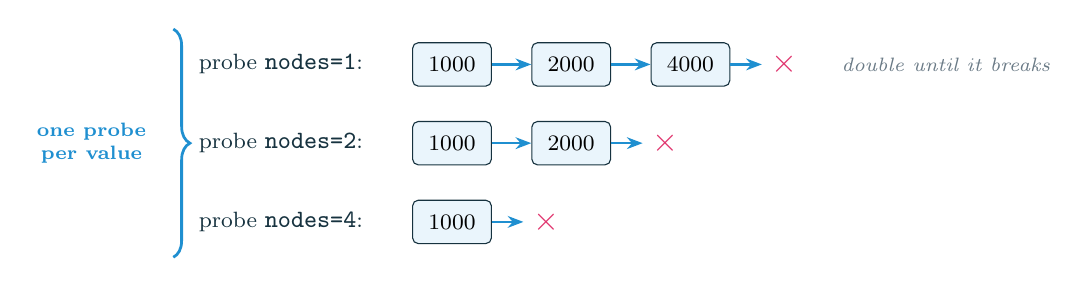
\begin{tikzpicture}[
      v/.style={rounded corners=2pt, draw=iopsNavy, fill=iopsSky,
        minimum width=1.0cm, minimum height=0.55cm, font=\footnotesize},
      a/.style={-{Stealth[length=2mm]}, color=iopsBlue, line width=0.8pt},
      lbl/.style={font=\footnotesize, color=iopsNavy, anchor=east},
      xx/.style={font=\large\bfseries, color=iopsPink}]
    % row 1: nodes=1
    \node[lbl] (l1) at (0,0) {probe \code{nodes=1}:};
    \node[v, right=5mm of l1] (a1) {1000};
    \node[v, right=5mm of a1] (a2) {2000};
    \node[v, right=5mm of a2] (a3) {4000};
    \node[xx, right=4mm of a3] (ax) {$\times$};
    \draw[a] (a1)--(a2); \draw[a] (a2)--(a3); \draw[a] (a3)--(ax);
    % row 2: nodes=2
    \node[lbl] (l2) at (0,-1) {probe \code{nodes=2}:};
    \node[v, right=5mm of l2] (b1) {1000};
    \node[v, right=5mm of b1] (b2) {2000};
    \node[xx, right=4mm of b2] (bx) {$\times$};
    \draw[a] (b1)--(b2); \draw[a] (b2)--(bx);
    % row 3: nodes=4
    \node[lbl] (l3) at (0,-2) {probe \code{nodes=4}:};
    \node[v, right=5mm of l3] (c1) {1000};
    \node[xx, right=4mm of c1] (cx) {$\times$};
    \draw[a] (c1)--(cx);
    % brace: one probe per nodes value
    \draw[decorate, decoration={brace, amplitude=6pt}, color=iopsBlue, line width=1pt]
      ($(l1.north west)+(-2mm,2mm)$) -- ($(l3.south west)+(-2mm,-2mm)$)
      node[midway, left=6pt, align=center, font=\scriptsize\bfseries, color=iopsBlue]
      {one probe\\per value};
    % step annotation
    \node[font=\scriptsize\itshape, color=iopsGrey, anchor=west] at ($(ax)+(6mm,0)$)
      {double until it breaks};
  \end{tikzpicture}
  \end{center}
  \vspace{0.4em}
  \begin{keybox}
    \faInfoCircle~Each probe steps its adaptive value independently until its
    \code{stop\_when} fires, finding the limit \emph{for that combination}.
  \end{keybox}
\end{frame}

\end{document}
